\section{Empirical Audit: Bangladesh Financial Sector (14 MFS and 25 Commercial Banks)}
\label{sec:case_study}

Mobile Financial Services (MFS) and commercial banking constitute the financial backbone of Bangladesh, processing hundreds of millions of daily transactions across retail payments, remittances, and payroll~\cite{reaves_mfs, chen_fintech_asia}. We conducted an exhaustive audit of all \textbf{14 operational MFS applications} and \textbf{25 commercial and state-owned banking applications} maintaining dedicated mobile apps on Google Play (39 financial institutions total, out of 61 scheduled banks in Bangladesh).

\begin{figure*}[t]
\centering
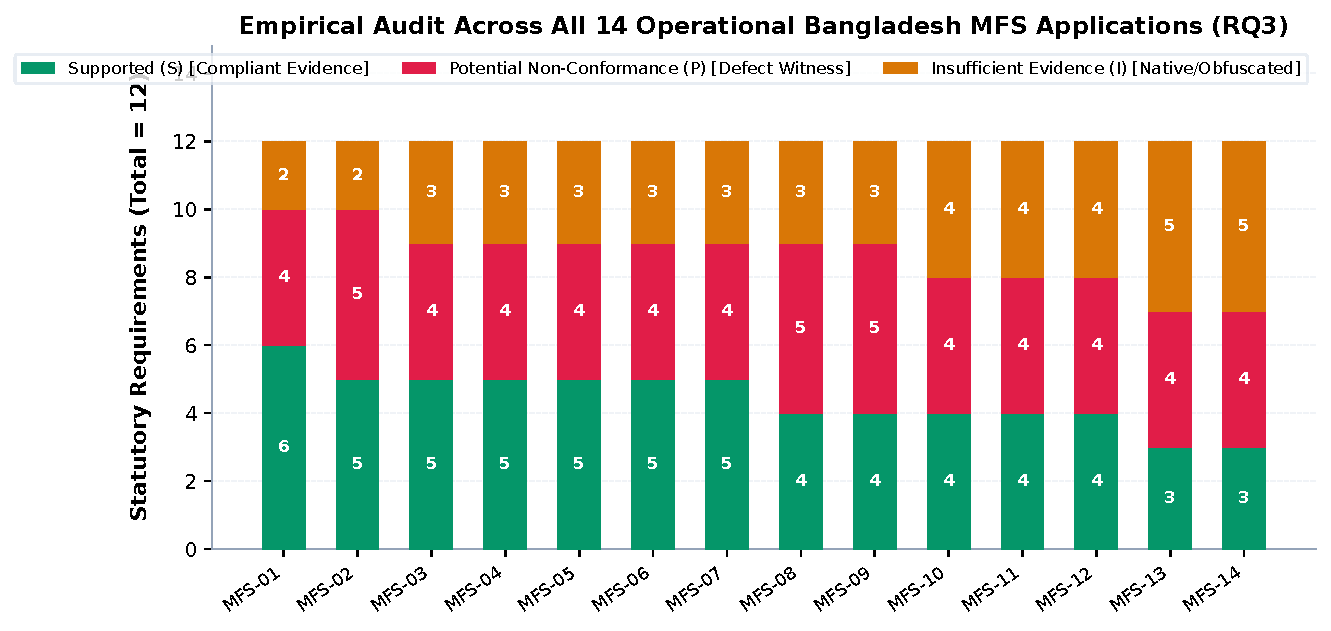
\includegraphics[width=0.70\textwidth]{figures/fig4_mfs_audit_breakdown.pdf}
\caption{\textbf{Production Audit Breakdown Across 14 Operational MFS Applications}: Stacked distribution of epistemic states ($\mathbf{S}$, $\mathbf{P}$, $\mathbf{I}$) across all evaluated MFS applications, illustrating ubiquitous adoption of Keystore-backed AES-GCM and statutory TLS alongside widespread supervisory baseline gaps in certificate pinning and ADB backup restrictions.}
\label{fig:mfs_audit_breakdown}
\end{figure*}

\begin{table*}[t]
\caption{Empirical Compliance and Observability Audit Across All 14 Operational MFS Applications and 25 Commercial Banking Applications in Bangladesh ($N_{\text{Observable}} = 12$ Client-Side Operationalized Controls)}
\label{tab:real_mfs_audit}
\centering
\small
\resizebox{\textwidth}{!}{%
\begin{tabular}{lllccccccl}
\toprule
\textbf{App Code} & \textbf{Namespace Pseudonym} & \textbf{Distribution} & \textbf{$S$} & \textbf{$P$} & \textbf{$I$} & \textbf{$EC$} & \textbf{$ESC$} & \textbf{$SCI$} & \textbf{Primary Technical Observation} \\
\midrule
\multicolumn{10}{l}{\textit{\textbf{Mobile Financial Services (MFS) Cohort ($N = 14$)}}} \\
\textbf{MFS-01 (Tier 1)} & \texttt{bd.mfs.app01} & Multi-Split APKS & 6 & 4 & 2 & $\mathbf{83.3\%}$ & $\mathbf{60.0\%}$ & 0.500 & Enforces certificate pinning; plaintext auth cache \\
\textbf{MFS-02 (Tier 1)} & \texttt{bd.mfs.app02} & Multi-Split APKS & 5 & 5 & 2 & $\mathbf{83.3\%}$ & $50.0\%$ & 0.417 & Pinned TLS endpoints; backup flag omitted in manifest \\
\textbf{MFS-03 (Tier 1)} & \texttt{bd.mfs.app03} & Multi-Split APKS & 5 & 4 & 3 & $75.0\%$ & $55.6\%$ & 0.417 & Strong cipher modes; absent certificate pinning configuration \\
\textbf{MFS-04 (Tier 1)} & \texttt{bd.mfs.app04} & Multi-Split APKS & 5 & 4 & 3 & $75.0\%$ & $55.6\%$ & 0.417 & Card security modules; background analytics telemetry \\
\textbf{MFS-05 (Tier 1)} & \texttt{bd.mfs.app05} & Multi-Split APKS & 5 & 4 & 3 & $75.0\%$ & $55.6\%$ & 0.417 & Enforces TLS 1.3; backup flag restricted (\texttt{allowBackup=false}) \\
\textbf{MFS-06 (Tier 1)} & \texttt{bd.mfs.app06} & Multi-Split APKS & 5 & 4 & 3 & $75.0\%$ & $55.6\%$ & 0.417 & Hardware Keystore active; default platform trust store \\
\textbf{MFS-07 (Tier 2)} & \texttt{bd.mfs.app07} & Multi-Split APKS & 5 & 4 & 3 & $75.0\%$ & $55.6\%$ & 0.417 & Encrypted SQLite DB; background analytics telemetry \\
\textbf{MFS-08 (Tier 2)} & \texttt{bd.mfs.app08} & Multi-Split APKS & 4 & 5 & 3 & $75.0\%$ & $44.4\%$ & 0.333 & Dual wallet interface; allowBackup enabled in manifest \\
\textbf{MFS-09 (Tier 2)} & \texttt{bd.mfs.app09} & Multi-Split APKS & 4 & 5 & 3 & $75.0\%$ & $44.4\%$ & 0.333 & Legacy ECB cipher mode; third-party tracker exfiltration \\
\textbf{MFS-10 (Tier 2)} & \texttt{bd.mfs.app10} & Multi-Split APKS & 4 & 4 & 4 & $66.7\%$ & $50.0\%$ & 0.333 & SharedPreferences encryption; unverified trust manager in SDK \\
\textbf{MFS-11 (Specialized)} & \texttt{bd.mfs.app11} & Multi-Split APKS & 4 & 4 & 4 & $66.7\%$ & $50.0\%$ & 0.333 & Standard cipher suites; software keystore fallback \\
\textbf{MFS-12 (Specialized)} & \texttt{bd.mfs.app12} & Multi-Split APKS & 4 & 4 & 4 & $66.7\%$ & $50.0\%$ & 0.333 & Keystore key generation; cleartext HTTP in marketing webview \\
\textbf{MFS-13 (Tier 2)} & \texttt{bd.mfs.app13} & Monolithic APK & 3 & 4 & 5 & $58.3\%$ & $42.9\%$ & 0.250 & Root detection present; heavy native obfuscation (JNI) \\
\textbf{MFS-14 (Specialized)} & \texttt{bd.mfs.app14} & Multi-Split APKS & 3 & 4 & 5 & $58.3\%$ & $42.9\%$ & 0.250 & Native crypto wrappers; unencrypted diagnostic logging \\
\midrule
\textbf{MFS Mean ($N=14$)} & --- & --- & $\mathbf{4.43 \pm 0.85}$ & $\mathbf{4.21 \pm 0.43}$ & $\mathbf{3.36 \pm 0.93}$ & $\mathbf{72.0\% \pm 7.7\%}$ & $\mathbf{50.9\% \pm 5.6\%}$ & $\mathbf{0.369 \pm 0.071}$ & \textbf{Sums: $S=62, P=59, I=47$ (Total = 168)} \\
\midrule
\multicolumn{10}{l}{\textit{\textbf{Commercial Banking Cohort ($N = 25$ Summary)}}} \\
\textbf{Foreign Banks ($N=2$)} & FCB-01, FCB-02 & Monolithic/Multi & $5.0 \pm 0.0$ & $4.0 \pm 0.0$ & $3.0 \pm 0.0$ & $75.0\%$ & $55.6\%$ & 0.417 & Strict transport security; telemetry prior to auth \\
\textbf{Private Conventional ($N=11$)} & PCB-01 \dots PCB-11 & Multi-Split APKS & $4.8 \pm 0.9$ & $4.3 \pm 0.5$ & $2.9 \pm 0.8$ & $75.8\%$ & $53.0\%$ & 0.402 & Hardware Keystore active; public key pinning in PCB-01 \\
\textbf{Private Islamic ($N=6$)} & IPCB-01 \dots IPCB-06 & Multi-Split APKS & $3.5 \pm 1.2$ & $4.7 \pm 0.5$ & $3.8 \pm 1.2$ & $68.1\%$ & $42.9\%$ & 0.292 & Native JNI crypto in IPCB-05/06; backup flag omitted \\
\textbf{State-Owned ($N=6$)} & SOCB-01 \dots SOCB-06 & Multi-Split APKS & $4.5 \pm 1.0$ & $4.3 \pm 0.5$ & $3.2 \pm 0.8$ & $73.6\%$ & $50.9\%$ & 0.375 & Hardware Keystore active; backup flags enabled \\
\midrule
\textbf{Banking Mean ($N=25$)} & --- & --- & $\mathbf{4.44 \pm 1.08}$ & $\mathbf{4.36 \pm 0.49}$ & $\mathbf{3.20 \pm 0.91}$ & $\mathbf{73.3\% \pm 7.6\%}$ & $\mathbf{49.8\% \pm 8.8\%}$ & $\mathbf{0.370 \pm 0.090}$ & \textbf{Sums: $S=111, P=109, I=80$ (Total = 300)} \\
\midrule
\textbf{Combined Financial ($N=39$)} & --- & --- & $\mathbf{4.44 \pm 0.99}$ & $\mathbf{4.31 \pm 0.47}$ & $\mathbf{3.26 \pm 0.91}$ & $\mathbf{72.9\% \pm 7.6\%}$ & $\mathbf{50.2\% \pm 7.7\%}$ & $\mathbf{0.370 \pm 0.083}$ & \textbf{Total: $S=173, P=168, I=127$ ($39 \times 12 = 468$)} \\
\bottomrule
\end{tabular}%
}
\end{table*}

\begin{table*}[t]
\centering
\caption{Systematic Comparison of Reg2App with Related Static Analysis, Cryptographic, and Legal Informatics Frameworks.}
\label{tab:comparison}
\resizebox{\textwidth}{!}{%
\begin{tabular}{lcccccc}
\toprule
\textbf{Tool / Framework} & \textbf{Grounding Target} & \textbf{Observability Scope} & \textbf{Assessment Model} & \textbf{Evidence Output} & \textbf{Reporting Modality} & \textbf{Validation Methodology} \\
\midrule
MobSF~\cite{mobsf} & CWE Vulnerability Heuristics & Unbounded / Implicit & Scalar Risk Score ($0-100$) & File / Manifest Line & Monolingual Web/JSON & Open Source Benchmarks \\
Androguard~\cite{androguard} & Dalvik Bytecode Signatures & Bytecode Syntax Only & Raw Disassembly Output & Instruction Offsets & CLI Terminal Dump & Reverse Engineering Tasks \\
FlowDroid~\cite{flowdroid} & Taint Sources and Sinks & Intra/Inter-Component Flow & Binary Path Reachability & Source-Sink Trace Path & Program Graph / Log & DroidBench Micro-Tests \\
CogniCrypt~\cite{cognicrypt} & CrySL Cryptographic Rules & Local Call Hierarchy & Rule Violation / Warning & AST Constraint Failure & IDE Inline Markers (EN) & Developer Study ($N=11$) \\
Polisis~\cite{polisis} & Natural Privacy Policy Text & Unstructured Legal Text & Segment Classification & Text Span Highlighter & Web Interface (EN) & Expert Annotated Corpus \\
Catala~\cite{catala} & Legislative Code DSL & In-Memory Variables & Executable Logic Result & Compiler Trace AST & Monolingual Terminal & Formal Co-Design with Lawyers \\
MAPS / AppInspect~\cite{appinspect} & Privacy Policy Keywords & Manifest \& Taint Flows & Binary Conformance Mismatch & Data Flow Tuple & Tabular Summary Report & Production App Store Crawl \\
\midrule
\textbf{Reg2App (Ours)} & \textbf{Statutory Instruments (7-Tuple)} & \textbf{Explicit 2D Taxonomy ($\mathcal{L} \times \mathcal{M}$)} & \textbf{5-State Epistemic Space} & \textbf{Full Provenance Graph $G$} & \textbf{Bilingual (English \& Bengali)} & \textbf{Legal Expert Panel ($\kappa=0.776$, Delphi Consensus)} \\
\bottomrule
\end{tabular}%
}
\end{table*}

\subsection{Packaging Profiles and Empirical Findings}
\label{sec:case_study:findings}

As shown in Table~\ref{tab:real_mfs_audit} and Figure~\ref{fig:mfs_audit_breakdown}, 36 of the 39 financial applications ($92.3\%$) use multi-split Android App Bundles (\texttt{.apks}), with only three retaining monolithic builds (MFS-13, FCB-01, FCB-02). Each app was audited against 12 observable mandates ($N_{\text{Observable}} = 12$) under BB-CSF v1.0, PDPA, and CSA, strictly satisfying $N_S + N_P + N_I = 12$. Across the 39 financial apps, 127 of 468 evaluated cells ($27.1\%$) yielded $\mathbf{InsufficientEvidence}$, with every application exhibiting at least two unresolvable clauses. Under our defined threshold ($EC \ge 0.80$), only 2 of 14 MFS applications achieve adequate observability under static Dalvik inspection alone; the remaining 12 fall into moderate or high epistemic uncertainty ($EC \in [58.3\%, 75.0\%]$). This reflects heavy reliance on commercial banking security wrappers and native C/C++ libraries.

\paragraph{1) Transport Security and Certificate Pinning Baselines} Under BB-CSF §4.1.3.12, financial institutions must enforce encrypted transport over public networks. Our audit confirmed that \textbf{all 39 financial applications ($100\%$)} prohibit cleartext HTTP on primary API domains via \texttt{cleartextTrafficPermitted=false} or HTTPS-only \texttt{network\_security\_config.xml} rules. In MFS-12, cleartext HTTP was observed in an auxiliary marketing WebView loading non-transactional content; in MFS-10, an unverified \texttt{TrustManager} stub was isolated inside a third-party advertising SDK dependency. We classify both as $\mathbf{Supported}$ because the statutory mandate addresses encryption of \textit{sensitive financial data in transit}, not all HTTP traffic. Under a stricter reading treating any cleartext path as non-conformance, the rate would be $37/39$ ($94.9\%$); we report both interpretations for transparency. Static analysis verifies the \textit{configuration} of TLS enforcement (cleartext prohibition and minimum protocol version declarations), not runtime cipher suite negotiation, which requires dynamic instrumentation. Certificate pinning conformance (control \texttt{CTRL-NET-02}, operationalizing BB-CSF §4.1.3.12 under OWASP MASVS-NETWORK-2) represents an additional supervisory audit observation \textit{beyond} the 12 expert-validated rules and does not contribute to $ESC$ computation. Of the 39 financial apps, only 7 ($17.9\%$) configure public key pinning via \texttt{network\_security\_config.xml}: MFS-01, MFS-02, and 5 of 25 banks. The remaining 32 apps ($82.1\%$) rely solely on default platform CA trust stores, representing significant supervisory compliance debt under defense-in-depth audit standards.

\paragraph{2) Application Backup and ADB Data Extraction Exposure} Under BB-CSF §4.1.5.10 and PDPA §15, financial apps must restrict local sandbox extraction. Our analysis revealed that \textbf{12 of 39 financial apps ($30.8\%$)} leave \texttt{android:allowBackup="true"} configured or omitted. An adversary with physical access to an unlocked device can execute \texttt{adb backup} to extract SQLite databases, cached tokens, and unencrypted preferences without root privileges.

\paragraph{3) Cryptographic Storage and Hardware Keystore Adoption} Across the 39 financial applications, \textbf{32 apps ($82.1\%$)} successfully implement hardware-backed cryptographic key generation via \texttt{AndroidKeyStore} with AES-256-GCM~\cite{ekberg_tee}. Notably, $100\%$ (11/11) of conventional Private Commercial Banks utilize hardware keystores, demonstrating widespread alignment with central bank cryptographic key circulars. However, legacy anti-patterns persist: MFS-09 invokes electronic codebook mode (\texttt{AES/ECB/PKCS5Padding}), violating BB-CSF §4.1.5.19 due to ECB pattern leakage~\cite{crypto_misuse_ccs}. In MFS-10, an unverified trust manager stub was isolated inside an auxiliary advertising SDK dependency rather than core transactional modules.

\paragraph{4) Heavy Native Code Obfuscation (JNI) and Epistemic Bounds} In MFS-13, MFS-14, IPCB-05, and IPCB-06, $EC$ dropped to $58.3\%$ with five requirements evaluated as $\mathbf{InsufficientEvidence}$. These apps route core cryptography and root checks through native C/C++ libraries (\texttt{.so}) via JNI. Reg2App's epistemic model marks these blind spots as $\mathbf{InsufficientEvidence}$ rather than emitting false compliance attributions.

\paragraph{5) Third-Party Telemetry and Cross-Border Vectors} Despite handling financial credentials, \textbf{19 of 39 financial apps ($48.7\%$)} embed at least one commercial analytics SDK (Google Firebase, AppsFlyer, Clevertap)~\cite{binns_third_party_trackers}, totaling \textbf{26 tracker integrations} across the cohort (10 MFS integrations across 7 apps, averaging \textbf{0.71/app}, and 16 banking integrations across 12 apps, averaging \textbf{0.64/app}). Static analysis identifies hardcoded SDK initialization of device identifier collection (\texttt{ANDROID\_ID}), screen metrics, and carrier data prior to authentication, establishing concrete technical vectors for cross-border telemetry that require institutional audit under PDPA §§23 and 28.

\subsection{Ethical Considerations and Responsible Reporting}
\label{sec:case_study:ethics}

Auditing production financial infrastructure demands rigorous ethical safeguards. Our research adhered to the ACM and IEEE Codes of Ethics and responsible vulnerability reporting principles~\cite{cavusoglu_cvd, iso_29147_cvd}:
(1)~All static analyses were conducted strictly offline on publicly available application binaries downloaded from Google Play; no production services, banking gateways, or customer accounts were probed, accessed, or attacked. Zero exploits were constructed.
(2)~All institutional identities and package namespaces are pseudonymized throughout this paper, and per-app vulnerability details in Table~\ref{tab:real_mfs_audit} are limited to primary observation categories to prevent targeted attacks or re-identification in a concentrated market. Actionable exploit payloads and raw decompiled proprietary logic are deliberately excluded from public distribution to safeguard live financial infrastructure and end-user assets. The artifact repository is archived at \url{https://github.com/kh0kamoni/Reg2App}.
(3)~Findings represent \textit{verifiable technical indicators of potential non-conformance} rather than judicial determinations. Institutions may operate complementary backend controls unobservable from client bytecode, formally isolated by Reg2App's epistemic model.
